\documentclass[10pt,twocolumn,letterpaper]{article}

\usepackage{cvpr}
\usepackage{times}
\usepackage{epsfig}
\usepackage{graphicx}
\usepackage{amsmath}
\usepackage{amssymb}
% Include other packages here, before hyperref.

% If you comment hyperref and then uncomment it, you should delete
% egpaper.aux before re-running latex.  (Or just hit 'q' on the first latex
% run, let it finish, and you should be clear).
\usepackage[breaklinks=true,bookmarks=false]{hyperref}

%\cvprfinalcopy % *** Uncomment this line for the final submission

\def\cvprPaperID{****} % *** Enter the CVPR Paper ID here
\def\httilde{\mbox{\tt\raisebox{-.5ex}{\symbol{126}}}}
% Pages are numbered in submission mode, and unnumbered in camera-ready
%\ifcvprfinal\pagestyle{empty}\fi
\setcounter{page}{1}
\begin{document}

%%%%%%%%% TITLE
\title{Freddie Mac Initial Data Analysis}

\author{Thomas Billman}
% For a paper whose authors are all at the same institution,
% omit the following lines up until the closing ``}''.
% Additional authors and addresses can be added with ``\and'',
% just like the second author.
% To save space, use either the email address or home page, not both

\maketitle
%\thispagestyle{empty}

%%%%%%%%% ABSTRACT

%%%%%%%%% BODY TEXT
\section{Introduction}

Freddie Mac holds a large portion of the United States of America's home mortgages. As such looking for trends in the values and performance of these loans is crucial. Our dataset consists of data collected at the time loans were issued and a calculated Net Present Value (NPV) that acts as a proxy for the total value of each loan. This paper summarizes a subset of the different variables found in the dataset. The dataset can be found on my GitHub at the following address:
https://tinyurl.com/ycpr8lrj

%-------------------------------------------------------------------------
\section{Variables}
\subsection{Credit Score}

Figure \ref{fig:CreditScoreSummary} shows us the summary statistics of Credit Score, and Figure \ref{fig:CreditScoreHist} shows us the distribution. This distribution is skewed left with many individuals in the 650 - 775 range. 

\subsection{First Payment}

Figure \ref{fig:FirstPaymentS} shows us the frequency table of the year and month the first payment was made for each loan.Figure \ref{fig:FirstPaymentB} shows us the distribution as a bar chart. This distribution shows us that most borrowers made their first payment in the first half of 1999 with a few outliers all the way out into 2004.

\subsection{First Time Home Buyer Flag}

Figure \ref{fig:FirstTimeHomeS} shows us the frequency table of the flag marking if the borrowers for each loan were first time home buyers. This shows that very few (~10\%) of the loans were from these borrowers. Another notable quality is the amount of unreported data (~33\%). Figure \ref{fig:FirstTimeHomeB} shows us the distribution as a bar chart. This shows the same data as the summary. 

\subsection{Loan Maturity Date}

Figure \ref{fig:MaturityS} shows us the frequency table of the date the loans will mature or end. This shows a large spike in early 2029, which would be 30 years from most of the loans' origination date. This makes sense, and like the previous variable we also have some outliers sprinkled around the surrounding years. Figure \ref{fig:FirstTimeHomeB} shows us the distribution as a bar chart. This shows the same data as the summary. 

\subsection{Metropolitan Statistical Area (MSA) Codes}

Figure \ref{fig:MSAS} shows us the frequency table of the MSA codes of these homes. The actual codes do not give a lot of pertinent information, but we can not the large count of those marked Other and NA. "Other" likely refers to rural homes not included in an MSA. Figure \ref{fig:MSAB} shows us the distribution as a bar chart. This shows the same data as the summary. 

\subsection{Mortgage Insurance Percentage}

Figure \ref{fig:MIS} shows us the summary statistics of the mortgage insurance percentages of the homes. It is interesting to note that the majority of homes do not require mortgage insurance and the large amount of underreporting. Figure \ref{fig:MIB} shows us the distribution as a histogram. This also shows us that the majority of mortgage insurance policies are in round percentages(10\%, 25\%, etc.).

\subsection{Number of Units}

Figure \ref{fig:MIS} shows us the summary statistics of the number of units each loan covers. It is interesting to note that the vast majority of loans cover just one loan, however there are some that go as high as covering four units. It is also worth noting that in this case there are very few NAs. Figure \ref{fig:MIB} shows us the distribution as a bar chart. 

\subsection{Occupancy Status}

Figure \ref{fig:OccS} shows us the frequency table of the occupancy status of each home. This shows that the vast majority of these homes are owner occupied, while there is a subset that are either investments or secondary homes. Figure \ref{fig:OccB} shows us the distribution as a bar chart. 

\subsection{Combined Loan to Value}

Figure \ref{fig:CLTVS} shows us the Combined Loan to Value Ratio of each home. This is the initial loan amount plus any lent to refinance divided by the cost of the home. This shows that most loans have a CLTV of around 80\%. Figure \ref{fig:CLTVB} shows us the distribution as a histogram. This shows us that many people try to get as close to 80\% as they can without going over. Usually going over requires mortgage insurance, which many borrowers prefer not to pay.

\subsection{Debt to Income Ratio}

Figure \ref{fig:DTIS} shows us the summary statistics of the Debt to Income Ratio of each loan. This is the percent of the borrower's income each month that is paid to the mortgage. Most of the data is in the 20-40\% range. Figure \ref{fig:DTIB} shows us the distribution as a histogram. This distribution is surprisingly very normal.

\subsection{Unpaid Balance}

Figure \ref{fig:UPBS} shows us the summary statistics of the initial unpaid balances of each loan. This is the same thing as the amount loaned. This shows that most loans at this time were around \$100,000. Figure \ref{fig:UPBB} shows us the distribution as a histogram. It is interesting that there is a sharp decrease around \$250,000. This is because Freddie Mac generally does not accept loans with balances over \$250,000.

\subsection{Interest Rate}

Figure \ref{fig:IRS} shows us the summary statistics of the interest rate of each loan. At this time most interest rates were around 6-7\%. Figure \ref{fig:IRB} shows us the distribution as a histogram. 

\subsection{Property Type}

Figure \ref{fig:PTS} shows us the frequency table of the property type of each home. This shows that the majority of the loans are for single family homes, planned units, and condominiums. Figure \ref{fig:PTB} shows us the distribution as a bar chart. 

\subsection{Number of Borrowers}

Figure \ref{fig:NOBS} shows us the summary statistics of the number of borrowers on each loan. This shows that the majority of loans actually have two borrowers. Figure \ref{fig:NOBB} shows us the distribution as a bar chart. 

\subsection{Net Present Value (NPV)}

Figure \ref{fig:NPVS} shows us the summary statistics of the NPV of each loan. The NPV is our proxy of how profitable a loan ended up being for the lender. This shows that most loans end up netting the lender around \$10,000 - \$20,000 over what a 30 year government bond would yield. Figure \ref{fig:NPVB} shows us the distribution as a histogram. This shows the high volatility associated with the NPVs of these loans. Additionally how far out the outlying data points are. 


%-------------------------------------------------------------------------

\pagebreak

%Credit Score
\begin{figure}
	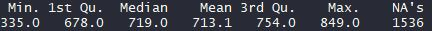
\includegraphics[width=0.45\textwidth]{images/CreditScoreSummary.JPG}
	\caption{Summary Statistics of Credit Score}
	\label{fig:CreditScoreSummary}
\end{figure}
\begin{figure}
	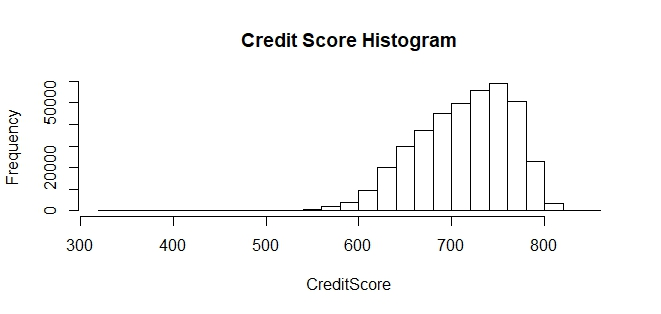
\includegraphics[width=0.45\textwidth]{images/CreditScoreHist.jpeg}
	\caption{Histogram of Credit Score}
	\label{fig:CreditScoreHist}
\end{figure}

%First Payment
\begin{figure}
	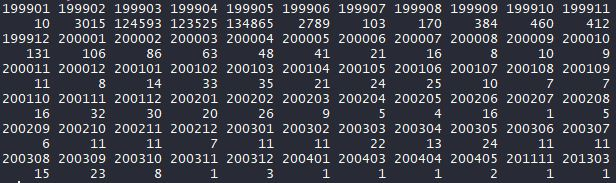
\includegraphics[width=0.45\textwidth]{images/FirstPaymentSummary.JPG}
	\caption{Frequency Table of First Payment}
	\label{fig:FirstPaymentS}
\end{figure}
\begin{figure}
	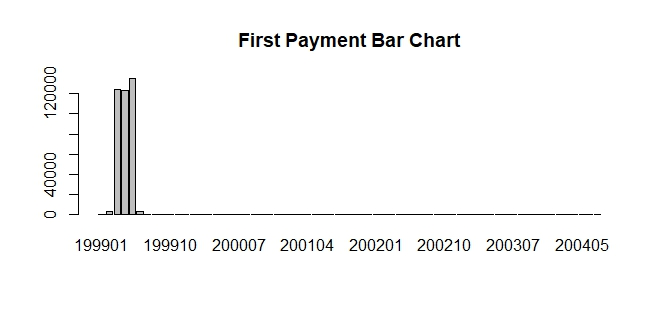
\includegraphics[width=0.45\textwidth]{images/FirstPaymentBarChart.jpeg}
	\caption{Histogram of Credit Score}
	\label{fig:FirstPaymentB}
\end{figure}

%FirstTimeHome
\begin{figure}
	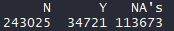
\includegraphics[width=0.45\textwidth]{images/FirstTimeHomeS.JPG}
	\caption{Frequency Table of First Time Home Buyers}
	\label{fig:FirstTimeHomeS}
\end{figure}
\begin{figure}
	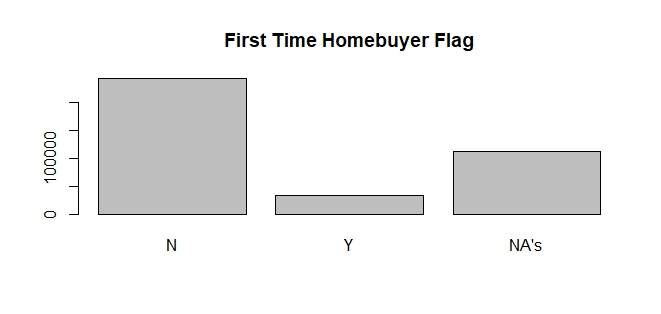
\includegraphics[width=0.45\textwidth]{images/FirstTimeHomeB.jpeg}
	\caption{Bar Chart of First Time Home Buyer Flag}
	\label{fig:FirstTimeHomeB}
\end{figure}

%Maturity
\begin{figure}
	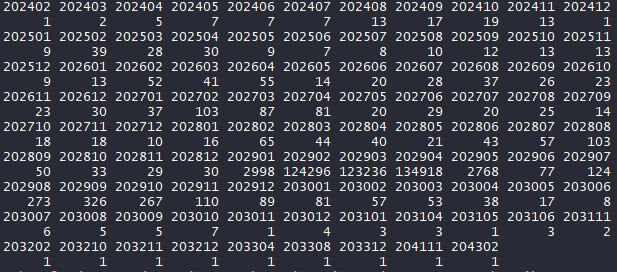
\includegraphics[width=0.45\textwidth]{images/MaturityS.JPG}
	\caption{Frequency Table of loan maturity date}
	\label{fig:MaturityS}
\end{figure}
\begin{figure}
	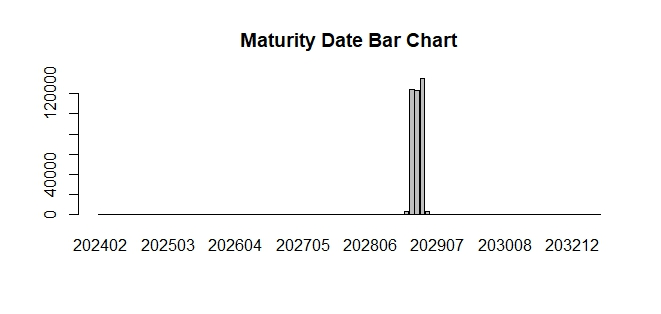
\includegraphics[width=0.45\textwidth]{images/MaturityB.jpeg}
	\caption{Bar Chart of loan maturity date}
	\label{fig:MaturityB}
\end{figure}

%MSA
\begin{figure}
	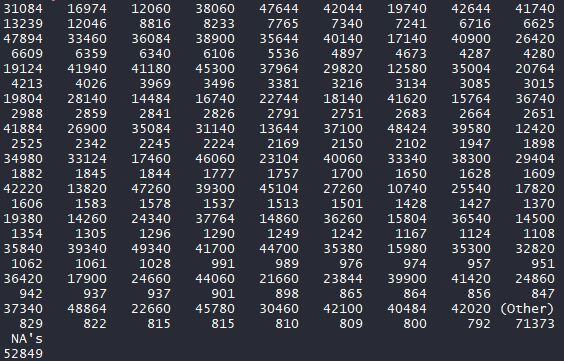
\includegraphics[width=0.45\textwidth]{images/MSAS.JPG}
	\caption{Frequency Table of Metropolitan Statistical Area locations}
	\label{fig:MSAS}
\end{figure}
\begin{figure}
	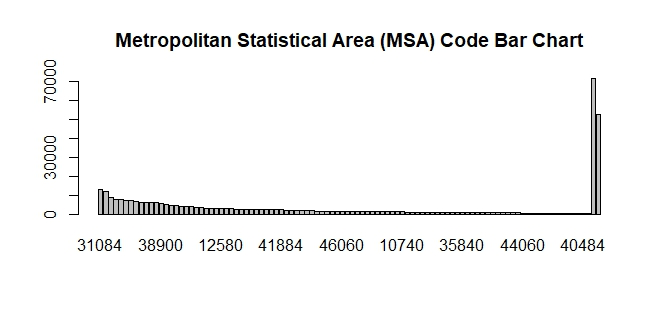
\includegraphics[width=0.45\textwidth]{images/MSAB.jpeg}
	\caption{Bar Chart of Metropolitan Statistical Area locations}
	\label{fig:MSAB}
\end{figure}

%MI
\begin{figure}
	\includegraphics[width=0.45\textwidth]{images/MIS.JPG}
	\caption{Summary Statistics of Mortgage Insurance Percentage}
	\label{fig:MIS}
\end{figure}
\begin{figure}
	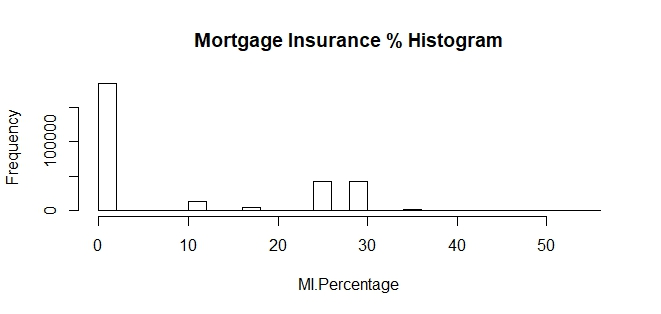
\includegraphics[width=0.45\textwidth]{images/MIB.jpeg}
	\caption{Bar Chart of Mortgage Insurance Percentage}
	\label{fig:MIB}
\end{figure}

%NOU
\begin{figure}
	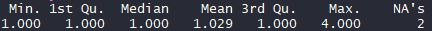
\includegraphics[width=0.45\textwidth]{images/NOUS.JPG}
	\caption{Frequency Table of Number of Units}
	\label{fig:NOUS}
\end{figure}
\begin{figure}
	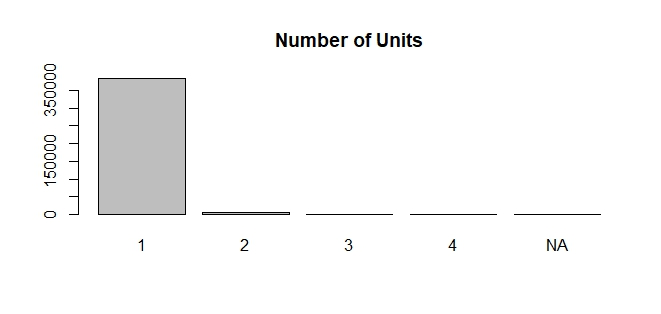
\includegraphics[width=0.45\textwidth]{images/NOUB.jpeg}
	\caption{Bar Chart of Number of Units}
	\label{fig:NOUB}
\end{figure}

%Occ
\begin{figure}
	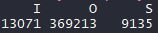
\includegraphics[width=0.45\textwidth]{images/OccS.JPG}
	\caption{Frequency Table of Occupancy Status}
	\label{fig:OccS}
\end{figure}
\begin{figure}
	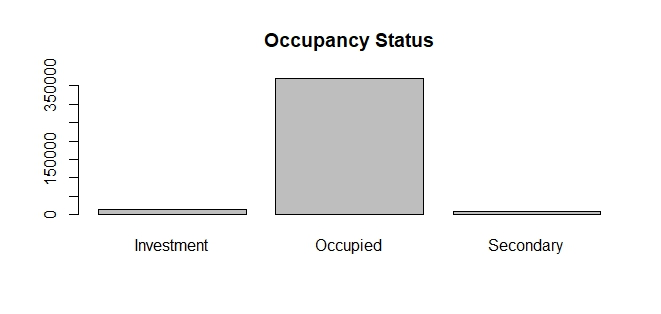
\includegraphics[width=0.45\textwidth]{images/OccB.jpeg}
	\caption{Bar Chart of Occupancy Status}
	\label{fig:OccB}
\end{figure}

%CLTV
\begin{figure}
	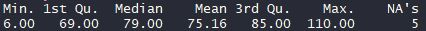
\includegraphics[width=0.45\textwidth]{images/CLTVS.JPG}
	\caption{Summary Statistics of Combined Loan to Value Ratio}
	\label{fig:CLTVS}
\end{figure}
\begin{figure}
	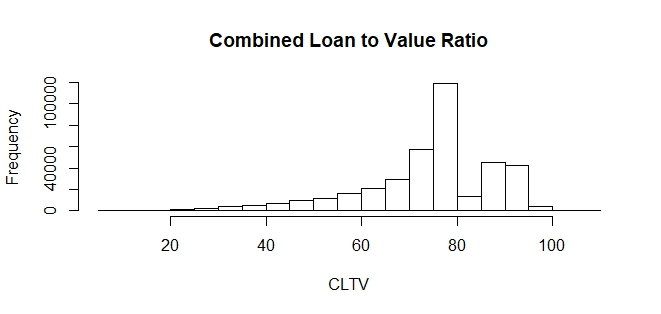
\includegraphics[width=0.45\textwidth]{images/CLTVB.jpeg}
	\caption{Histogram of Combined Loan to Value Ratio}
	\label{fig:CLTVB}
\end{figure}

%DTI
\begin{figure}
	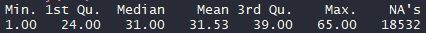
\includegraphics[width=0.45\textwidth]{images/DTIS.JPG}
	\caption{Summary Statistics of Debt to Income Ratio}
	\label{fig:DTIS}
\end{figure}
\begin{figure}
	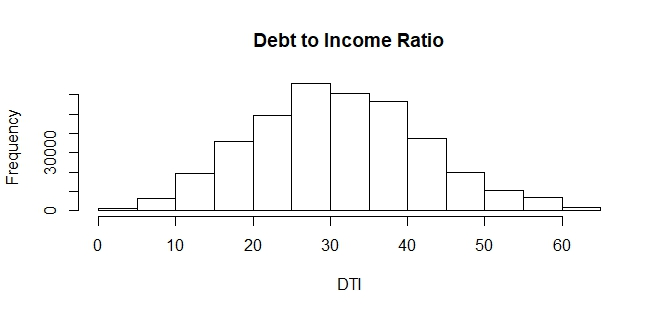
\includegraphics[width=0.45\textwidth]{images/DTIB.jpeg}
	\caption{Histogram of Debt to Income Ratio}
	\label{fig:DTIB}
\end{figure}

%UPB
\begin{figure}
	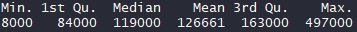
\includegraphics[width=0.45\textwidth]{images/UPBS.JPG}
	\caption{Summary Statistics of Unpaid Balance}
	\label{fig:UPBS}
\end{figure}
\begin{figure}
	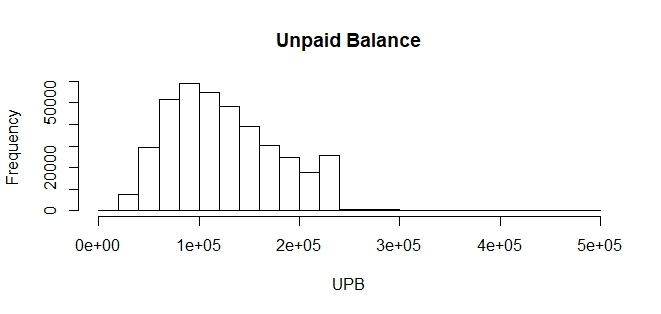
\includegraphics[width=0.45\textwidth]{images/UPBB.jpeg}
	\caption{Histogram of Unpaid Balance}
	\label{fig:UPBB}
\end{figure}

%IR
\begin{figure}
	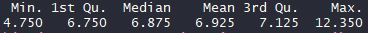
\includegraphics[width=0.45\textwidth]{images/IRS.JPG}
	\caption{Summary Statistics of Interest Rate}
	\label{fig:IRS}
\end{figure}
\begin{figure}
	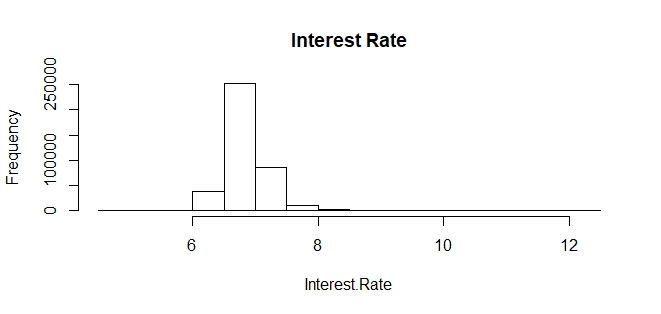
\includegraphics[width=0.45\textwidth]{images/IRB.jpeg}
	\caption{Histogram of Interest Rate}
	\label{fig:IRB}
\end{figure}

%PT
\begin{figure}
	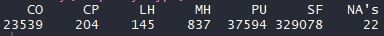
\includegraphics[width=0.45\textwidth]{images/PTS.JPG}
	\caption{Summary Statistics of Property Type}
	\label{fig:PTS}
\end{figure}
\begin{figure}
	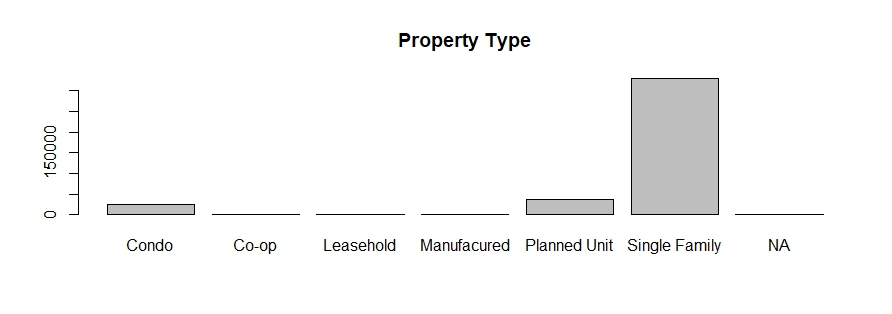
\includegraphics[width=0.45\textwidth]{images/PTB.jpeg}
	\caption{Bar Chart of Property Type}
	\label{fig:PTB}
\end{figure}

%NOB
\begin{figure}
	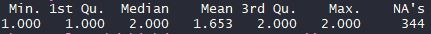
\includegraphics[width=0.45\textwidth]{images/NOBS.JPG}
	\caption{Summary Statistics of Number of Borrowers}
	\label{fig:NOBS}
\end{figure}
\begin{figure}
	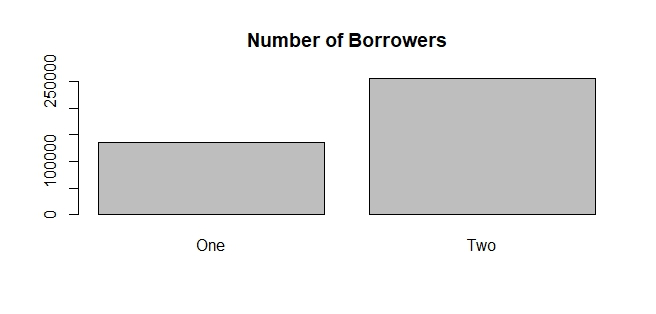
\includegraphics[width=0.45\textwidth]{images/NOBB.jpeg}
	\caption{Bar Chart of Number of Borrowers}
	\label{fig:NOBB}
\end{figure}

%NPV
\begin{figure}
	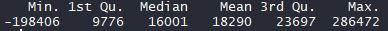
\includegraphics[width=0.45\textwidth]{images/NPVS.JPG}
	\caption{Summary Statistics of Net Present Value}
	\label{fig:NPVS}
\end{figure}
\begin{figure}
	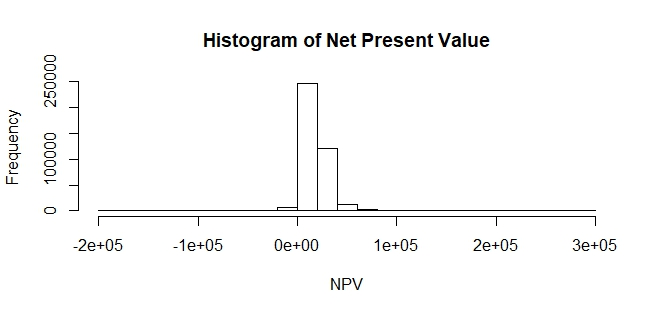
\includegraphics[width=0.45\textwidth]{images/NPVB.jpeg}
	\caption{Histogram of Net Present Value}
	\label{fig:NPVB}
\end{figure}



\end{document}
